\documentclass[12pt]{article}

% Fast build toggle: \draftbuildtrue = images replaced with boxes (quick)
%                    \draftbuildfalse = full images rendered (final PDF)
\newif\ifdraftbuild
\draftbuildfalse

\ifdraftbuild
  \PassOptionsToPackage{draft}{graphicx}
\fi
\usepackage{graphicx}
\usepackage{amsmath, amssymb}
\usepackage[margin=1in]{geometry}
\usepackage{fancyhdr}
\usepackage{enumerate}
\usepackage[shortlabels]{enumitem}
\usepackage[dvipsnames]{xcolor}
\usepackage{soul}
\usepackage{multicol}
\usepackage{color, colortbl}
\usepackage{geometry}
\usepackage{lastpage}
\usepackage{caption}
\captionsetup{font=it, labelsep=period}
\renewcommand{\figurename}{Fig.}
\usepackage{url}
\usepackage{setspace}
\usepackage{outlines}
\usepackage{placeins}
\usepackage{verbatim}
\usepackage{multirow}
\usepackage{float}
\usepackage{longtable}
\usepackage[breaklinks]{hyperref}

\setlength{\headheight}{14.5pt}
\addtolength{\topmargin}{-2.5pt}

\setcounter{tocdepth}{4}

\fontfamily{time}

\graphicspath{{./images/}{./Images/}}

% Paragraph formatting
\setlength{\parindent}{0pt}
\setlength{\parskip}{6pt}

\pagestyle{fancy}

\fancyhead[l]{WRIT 340}
\fancyhead[c]{White Paper}
\fancyhead[r]{Spring 2026}

\fancyfoot[l]{\raisebox{-0.3\height}{
\includegraphics[height=25pt]{images/TheShield.png}}}
\fancyfoot[c]{Page {\thepage} of {\pageref{LastPage}}}
\fancyfoot[r]{66837}

\renewcommand{\contentsname}{Table of Contents}  

\begin{document}
    \nocite{IEEEexample:BSTcontrol}
    \thispagestyle{fancy}
    \begin{center}
        \setlength{\headheight}{25pt}
        \vspace{0.3in}
        
\includegraphics[width=0.40\textwidth]{images/TheSeal_Reg_0921.png}\\
        \vspace{0.35in}
        \Huge {\textbf{Improving Accountability in \\Los Angeles Transit \\Infrastructure}}\\
        \vspace{0.4in}
        \Large {\textbf{WRIT 340}}\\
        \vspace{0.5in}
        \large {Jean Liang}\\
        \normalsize {jeanlian@usc.edu}\\
        \vspace{0.2in}
        \large {Nicole Popenko}\\
        \normalsize {popenko@usc.edu}\\
        \vspace{0.2in}
        \large {Philbert Loekman}\\
        \normalsize {ploekman@usc.edu}\\
        \vspace{0.5in}
        \Large {\textbf{Spring 2026}}\\
        \vspace{0.15in}
        \large {66837}\\
    \end{center}

    \newpage
    \pagestyle{fancy}

    \tableofcontents

    \newpage
    \listoffigures

    \newpage
    \section{Executive Summary}

    \newpage
    \section{Introduction}

    Los Angeles is undertaking one of the largest public transportation expansions in the United States, driven by voter-approved funding measures such as Measure R and Measure M. These initiatives represent a long-term commitment of over \$120 billion to improve regional mobility, reduce congestion, and support economic growth. Given the scale and importance of these investments, the successful delivery of transportation infrastructure is critical to the city's future.

    However, the implementation of these projects has been consistently challenged by cost overruns, delays, and discrepancies between projected and actual outcomes. These issues raise concerns not only about financial efficiency but also about the effectiveness of current planning and oversight processes. When projects fail to meet expectations, the consequences extend beyond budgetary concerns, affecting public trust and the credibility of future infrastructure initiatives.

    This white paper examines the structural factors that contribute to these recurring challenges. It focuses on three key issues: inaccuracies in cost estimation, the lack of enforceable cost controls after project approval, and delays resulting from insufficient accountability during project execution. It then proposes targeted solutions aimed at improving transparency, strengthening financial discipline, and ensuring that transportation investments deliver their intended outcomes.

    \newpage
    \section{Background}

    Despite the scale of investment in Los Angeles' transportation system, the region has experienced a consistent pattern of underperformance in delivering large-scale infrastructure projects. Several high-profile projects illustrate these challenges and provide insight into the systemic issues affecting project development.

    The California High-Speed Rail project, approved by voters in 2008, was initially estimated to cost approximately \$33 billion and intended to connect Northern and Southern California. Today, projected costs have increased to over \$126 billion, and no fully operational segment has been completed. Similarly, the LAX Automated People Mover (APM), designed to connect Los Angeles International Airport to regional transit and parking facilities, was originally budgeted at \$1.9 billion with a planned completion date of 2023. The project's cost has since grown to over \$3.34 billion, with an additional \$880 million in contractor-related settlement disputes, and it remains unfinished without a confirmed opening date.

    These examples are not isolated but reflect broader systemic patterns in how infrastructure projects are conceived and managed. In many cases, initial cost estimates are presented before sufficient technical information is available, timelines are influenced by political commitments, and mechanisms for enforcing budget and schedule discipline are limited. As a result, projects often begin with unrealistic expectations and encounter significant challenges during execution.

    At the same time, the demand for effective public transportation in Los Angeles continues to grow. Persistent traffic congestion, increasing population demands, and the approach of major international events such as the 2026 FIFA World Cup and the 2028 Olympic Games place additional pressure on the region's transit system to perform. To successfully build a public transportation network in Los Angeles in the future, it is important to understand these failures and why they occurred.

    \newpage
    \section{Problem}

        \subsection{}

        \subsection{Unchecked Cost Overruns in Transit Projects}

        Cost overruns that expand beyond initial voter or board approval represent a major source of waste in Los Angeles transportation infrastructure. Once a project secures funding through a ballot measure or board vote, agencies are generally permitted to absorb additional costs without returning to voters. This removes a critical check on government spending.

        The scale of this problem in Los Angeles is significant because of how local transit is funded. More than half of LA Metro's annual revenue comes from voter-approved sales taxes, primarily Measure R (a 0.5\% sales tax approved by LA County voters in 2008) and Measure M (an additional 0.5\% sales tax approved in 2016) \cite{p1}. Both measures listed specific projects with specific cost estimates on the ballot, but neither requires Metro to return to voters when those costs grow. As a result, the figures presented to voters at the ballot box rarely reflect what projects ultimately cost to build.

        This dynamic is reinforced at the federal level as well. Many LA Metro projects are partly paid for through the Federal Transit Administration's New Starts program, a competitive grant program that funds new rail and bus rapid transit projects across the country. Research on New Starts projects has consistently identified an ``optimism bias'' in the cost estimates agencies submit to win funding, meaning estimates tend to be systematically lower than what projects actually cost \cite{p2}. A study published in the Journal of the American Planning Association found that this bias is institutional rather than incidental because agencies have organizational incentives to produce forecasts that promote the project rather than accurate forecasts \cite{p3}.

        \begin{figure}[H]
            \centering
            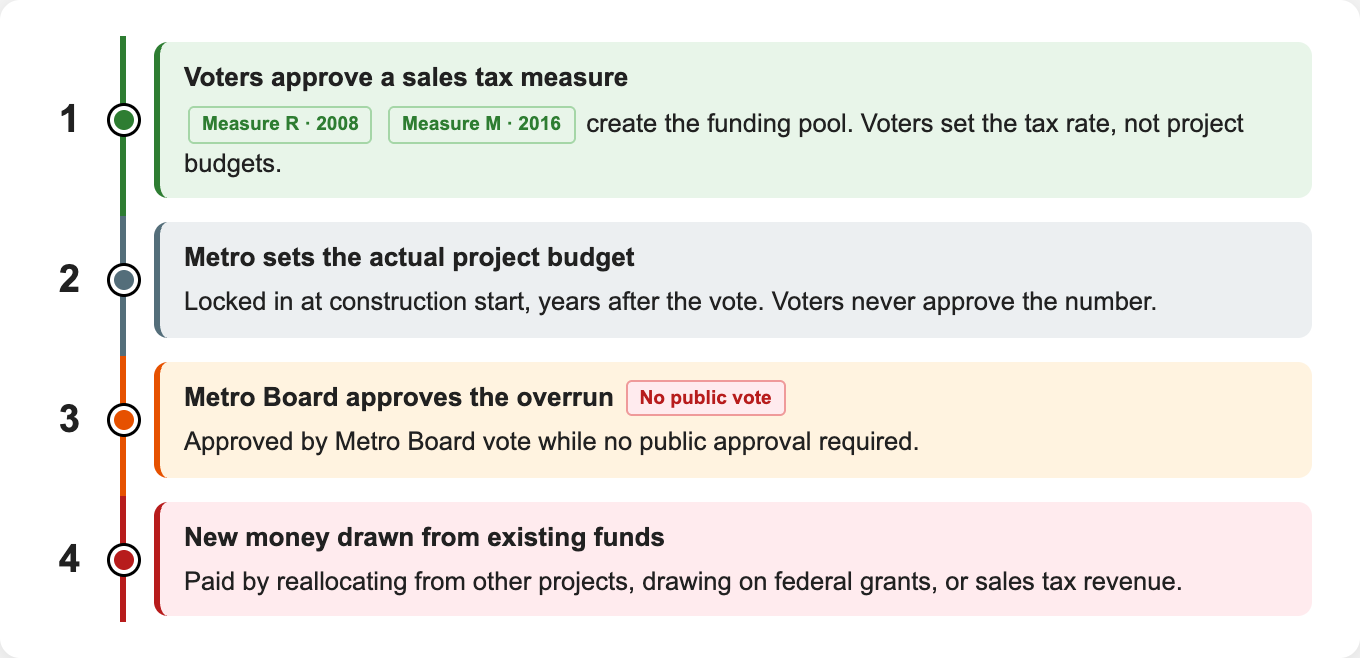
\includegraphics[width=\textwidth,keepaspectratio]{images/philbert/funding_flow_v1.png}
            \caption[How a Cost Overrun Moves Through LA Transit Funding]{How a Cost Overrun Moves Through LA Transit Funding: Voters approve the tax pool but never approve project budgets, allowing Metro to absorb overruns through internal board votes without returning to the public.}
            \label{fig:p4-funding-flow}
        \end{figure}

        The U.S. Government Accountability Office, the federal agency that audits how government money is spent, reached a similar conclusion. Its review of U.S. rail transit projects found that overruns are systematically tied to initial cost estimates being set too low and that current federal oversight does not adequately limit post-approval budget increases \cite{p4}. As a result, projects in Los Angeles frequently start construction with budgets that are known to be unreliable. This resulted in overruns being normalized as a standard behavior for projects rather than treated as failures. The structural pipeline that allows this to happen is shown in Fig.~\ref{fig:p4-funding-flow}, where voter approval of a tax pool is separated from the project budgets that actually spend it.

        \subsubsection{Case 1: D Line Subway Extension}

        \begin{figure}[H]
            \centering
            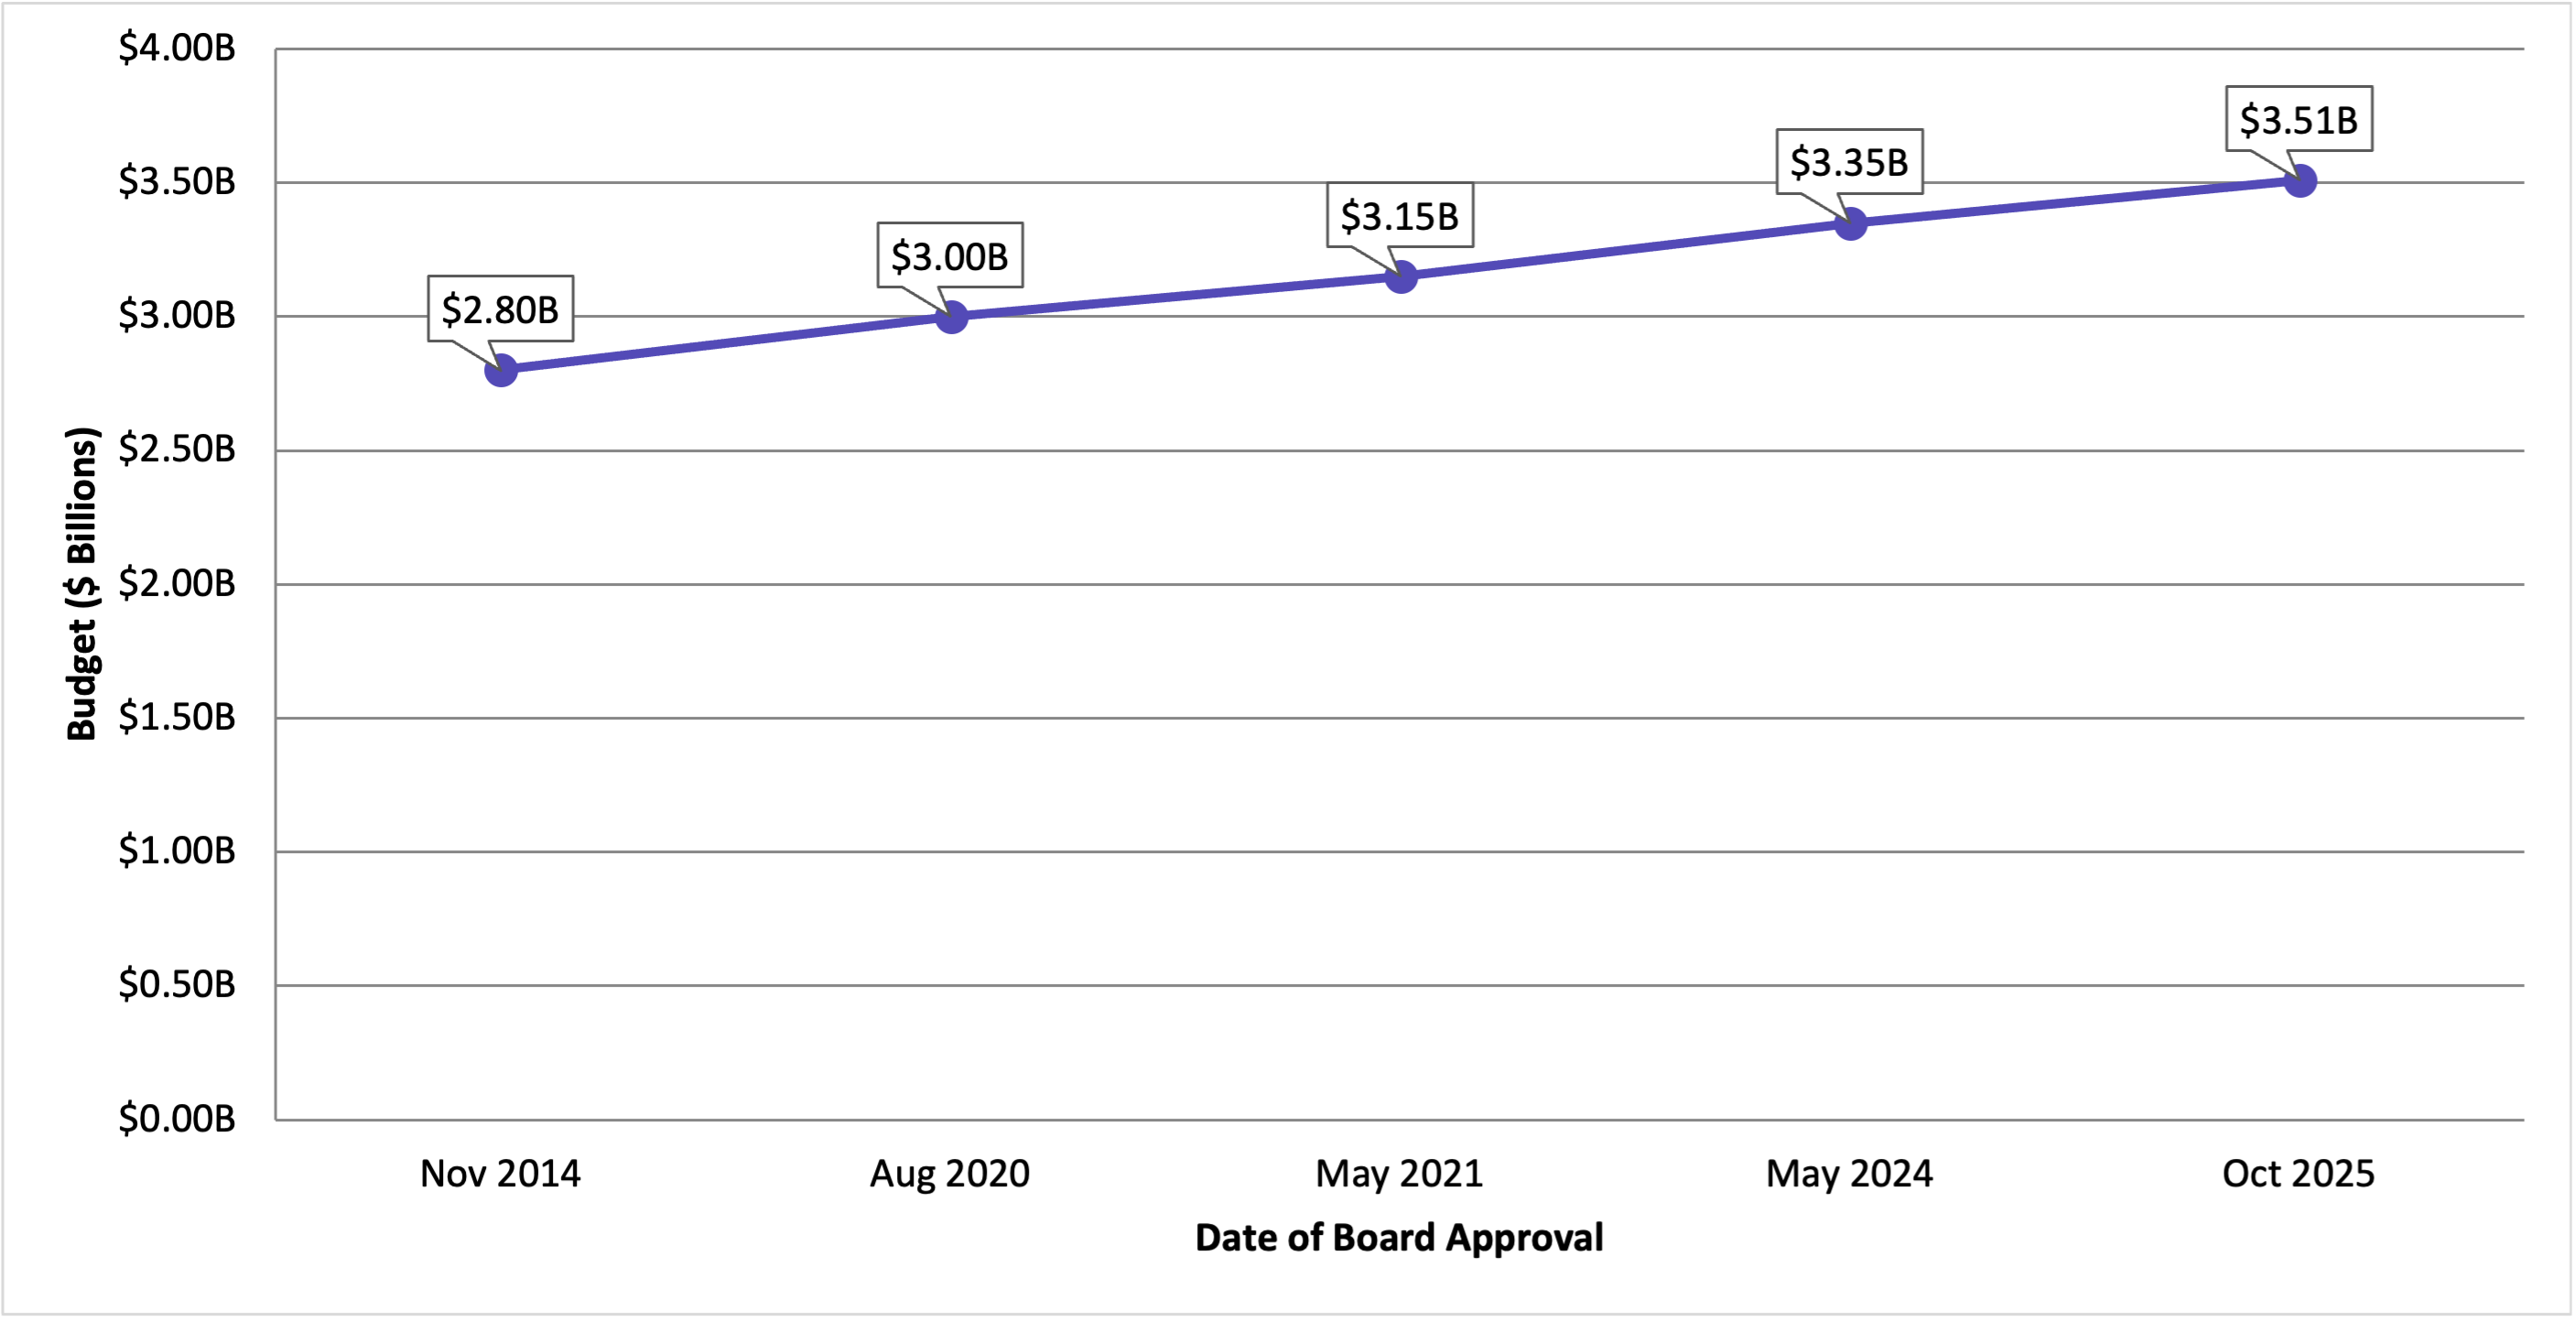
\includegraphics[width=\textwidth,keepaspectratio]{images/philbert/fig-p1-dline.png}
            \caption[D Line Section 1 Budget Over Time]{D Line Section 1 Budget Over Time: Budget grew from \$2.80 billion to \$3.51 billion between 2014 and 2025, a 25\% increase across four Metro Board votes with no voter re-authorization \cite{p11}.}
            \label{fig:p1-dline}
        \end{figure}

        This pattern of unchecked post-approval cost growth is evident in several major Los Angeles transportation projects. The Westside Subway Extension, also known as Section 1 of the D Line (Purple Line), was originally budgeted at approximately \$2.80 billion when construction began in 2014. Since then, the Metro Board has approved multiple cost increases without a public revote, raising the projected total to roughly \$3.51 billion (as shown in Fig.~\ref{fig:p1-dline}) \cite{p1, p11}.

        \subsubsection{Case 2: LAX Automated People Mover (APM)}

        \begin{figure}[H]
            \centering
            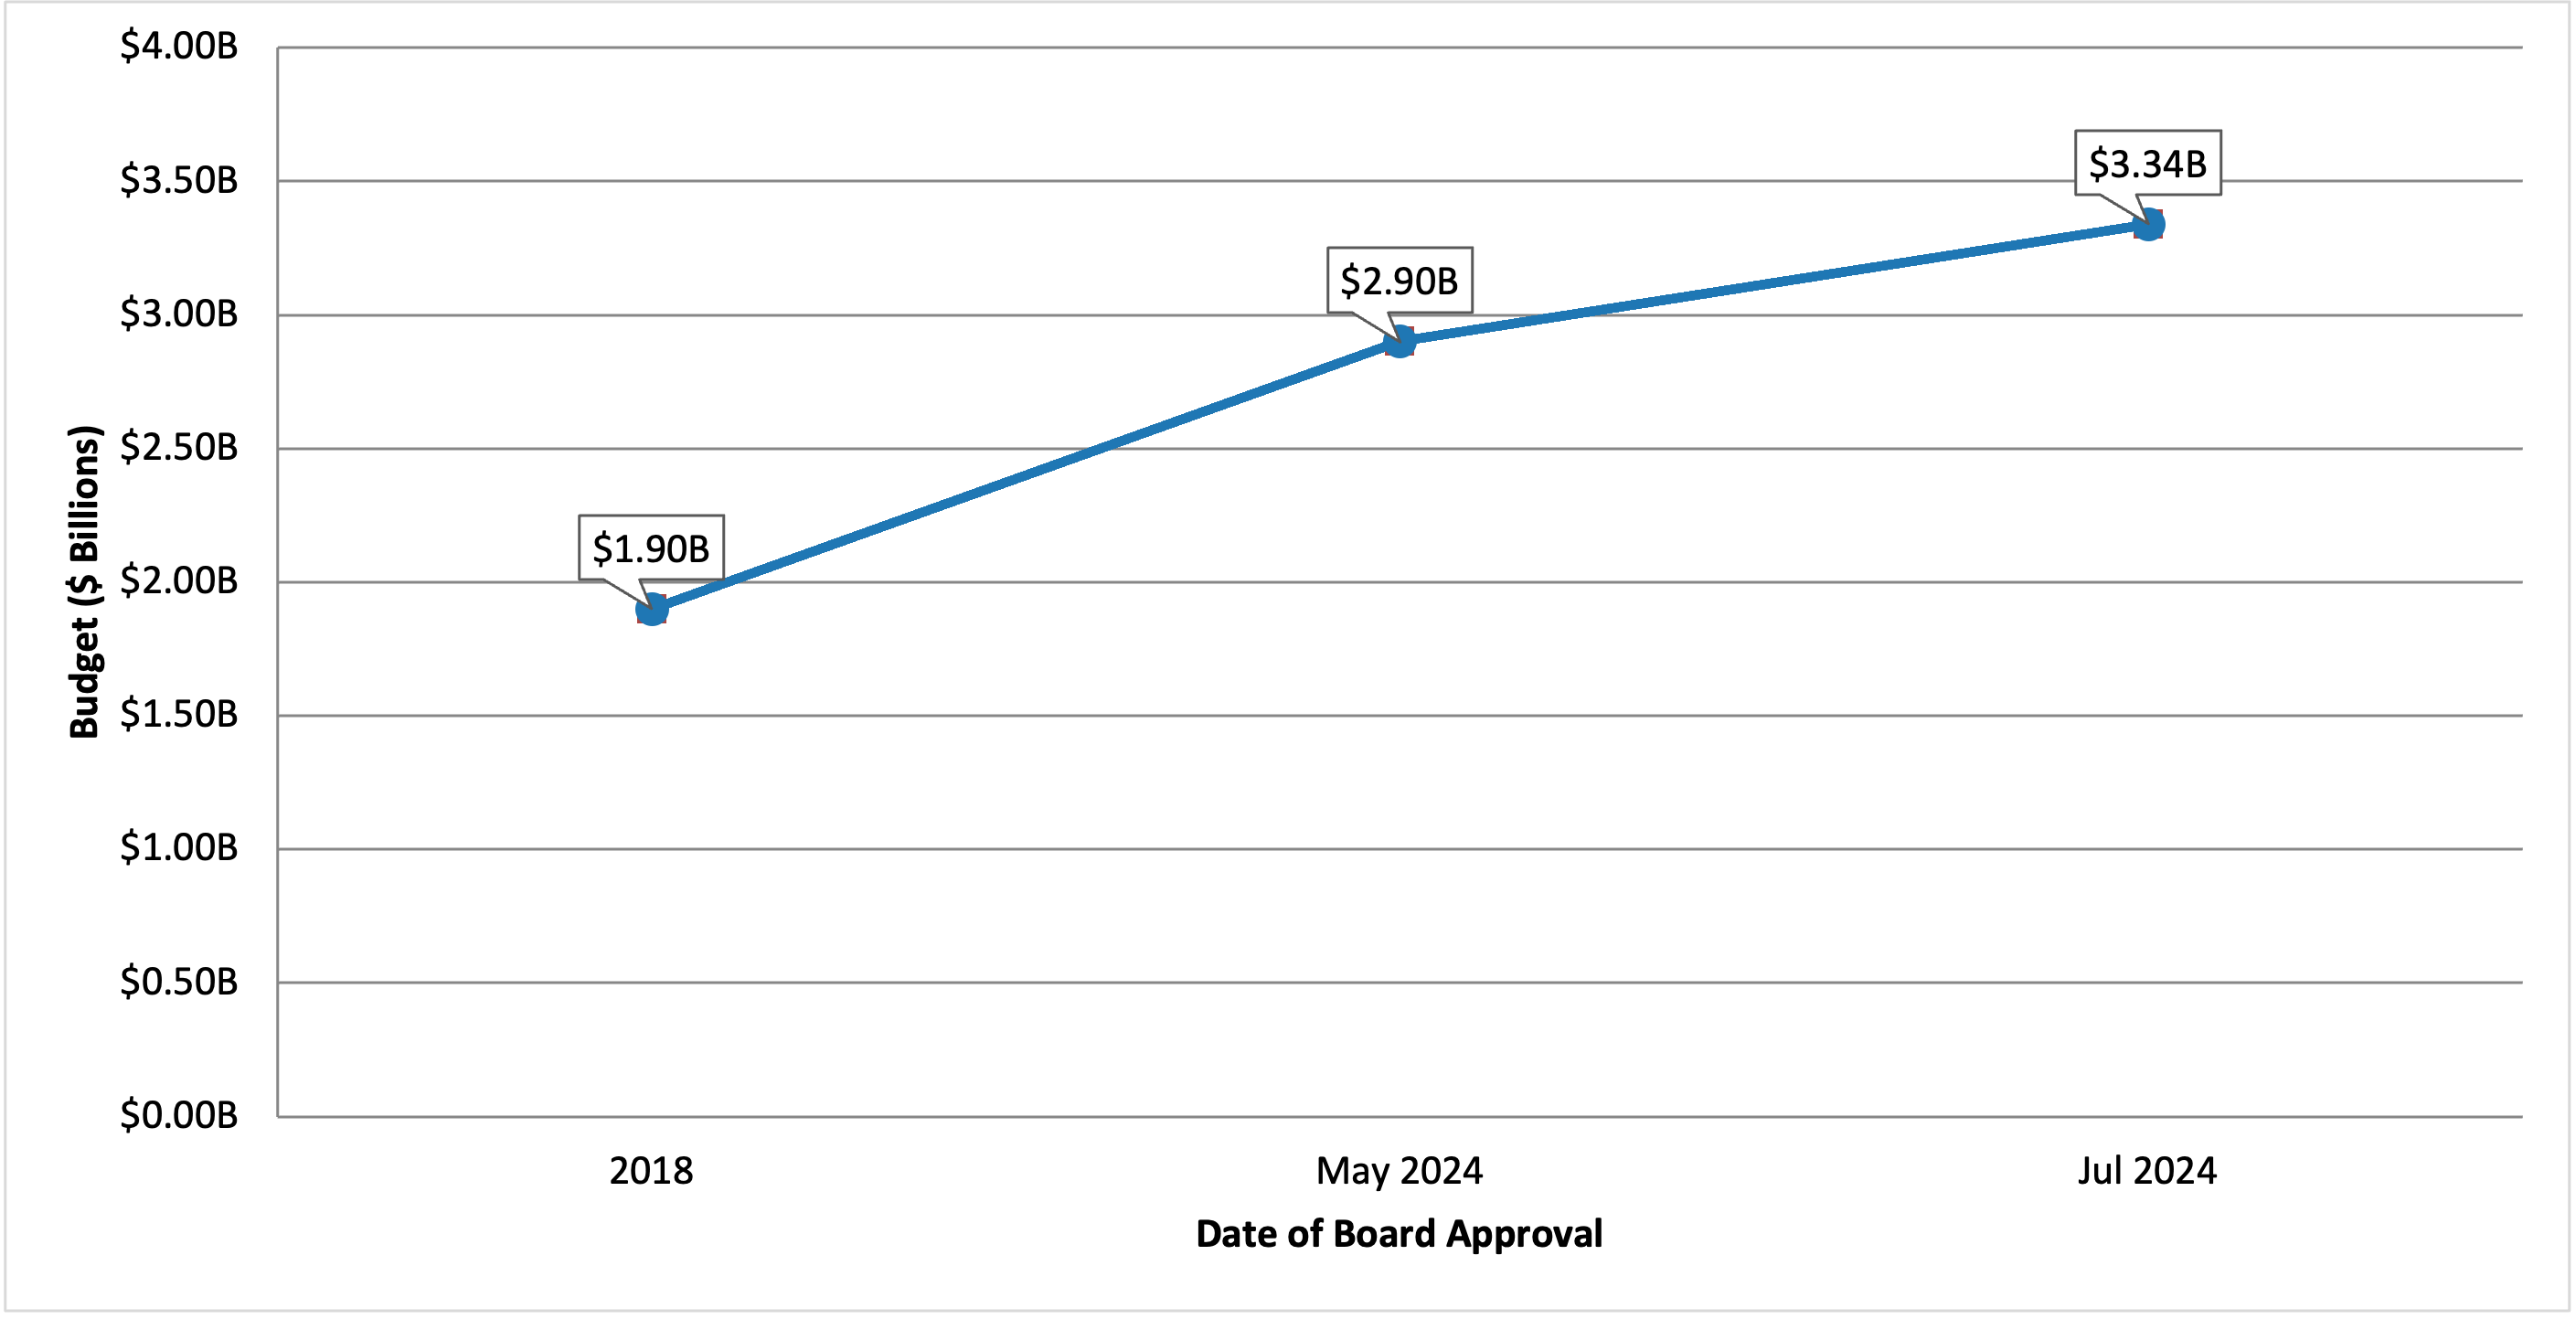
\includegraphics[width=\textwidth,keepaspectratio]{images/philbert/fig-p2-lax-apm.png}
            \caption[LAX Automated People Mover Budget Over Time]{LAX Automated People Mover Budget Over Time: Budget grew from \$1.90 billion to \$3.34 billion between 2018 and 2024, a 76\% increase, with an additional \$880 million in contractor disputes still unresolved \cite{p12, p13, p14}.}
            \label{fig:p2-lax-apm}
        \end{figure}

        The LAX Automated People Mover, the elevated train system being built to connect Los Angeles International Airport to nearby parking and transit, was originally estimated at \$1.9 billion. Today its cost has grown to \$3.34 billion, with an additional \$880 million in contractor settlement disputes, despite the fact that the project remains unfinished as of early 2026 (as shown in Fig.~\ref{fig:p2-lax-apm}) \cite{p5}.

        \subsubsection{Case 3: California High-Speed Rail}

        \begin{figure}[H]
            \centering
            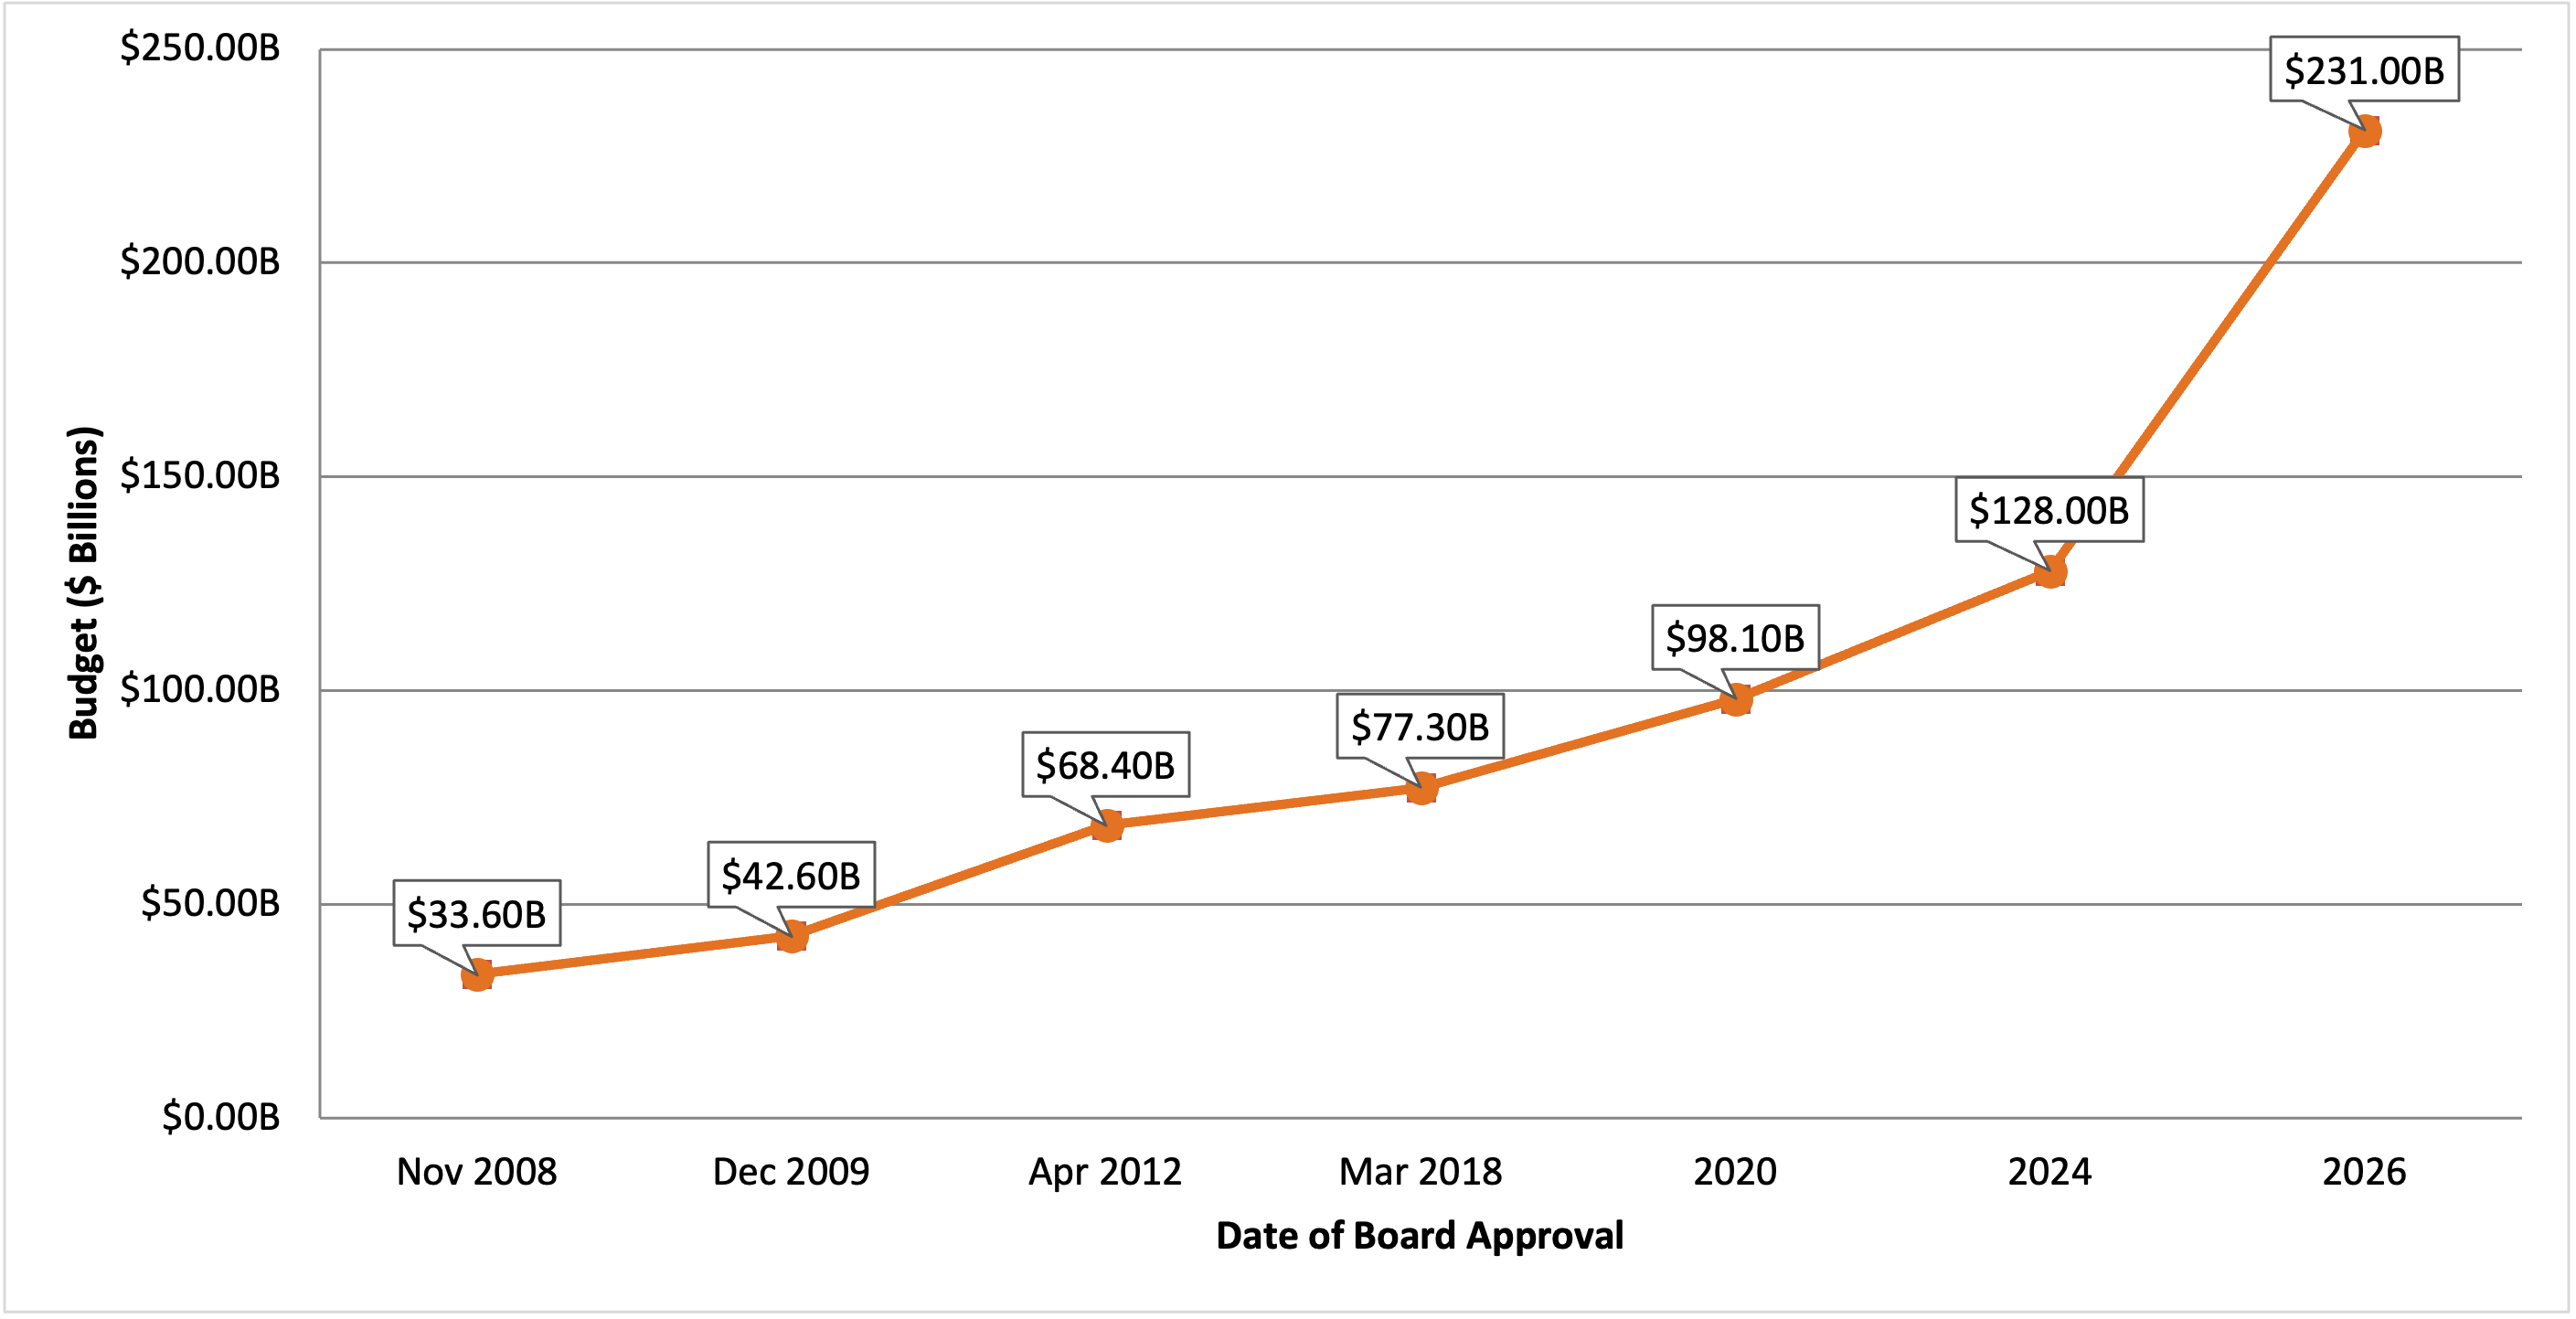
\includegraphics[width=\textwidth,keepaspectratio]{images/philbert/fig-p3-cahsr.png}
            \caption[California High-Speed Rail (Phase 1) Budget Over Time]{California High-Speed Rail (Phase 1) Budget Over Time: Cost estimate grew from \$33.6 billion to \$231 billion between 2008 and 2026, a 588\% increase, with no track segments operational \cite{p15, p16, p17, p18}.}
            \label{fig:p3-cahsr}
        \end{figure}

        At the state level, the California High-Speed Rail project provides the clearest example of what happens when large infrastructure is approved without binding cost limits. In 2008, California voters authorized a \$9.95 billion bond to support the project, which was then estimated at approximately \$33 billion in total (as shown in Fig.~\ref{fig:p3-cahsr}) \cite{p6, p18}. The projected total cost has since escalated to over \$231 billion, and no track segments are operational \cite{p6, p18}. The Government Accountability Office found that this escalation was facilitated in part by the absence of an independent cost estimation requirement at the federal level for high-speed rail, which allowed initial figures to advance without external verification \cite{p6}.

        Together, these cases demonstrate that without enforceable cost ceilings, projects are able to expand far beyond the financial commitments originally made to voters.

        \subsection{}

    \newpage
    \section{Solutions}

        \subsection{}

        \subsection{Voter-Approved Cost Caps}

        To address the issue of unchecked cost expansion after project approval, Los Angeles voter-approved transportation measures should be required to include legally binding cost caps for each major project listed in the expenditure plan. A cost cap is a maximum allowable budget assigned to a project at the time of voter approval. It would be calculated as the independently verified cost estimate plus a defined contingency percentage to account for reasonable construction risk such as weather delays or material price changes.

        If projected or actual costs exceed this cap by a predetermined threshold, project funding would be automatically suspended. From there, one of two outcomes would be required to continue the project:
        \begin{enumerate}
            \item A public ballot re-authorization for any budget increase
            \item For smaller breaches, a formal public hearing followed by a supermajority vote of the Metro Board of Directors
        \end{enumerate}

        This creates a structural stopping point that does not currently exist.

        This mechanism aligns with the research on accountability in megaprojects, which finds that meaningful cost discipline is achieved only when financial commitments are tied to enforceable approval gates rather than advisory oversight \cite{p7}.

        Implementation in Los Angeles should be paired with regulatory amendments to Measure M and any successor ballot measures. These amendments would require that all major capital projects above a defined cost threshold be subject to the cap mechanism. Compliance would be verified by an independent oversight body that operates separately from LA Metro's internal Office of Inspector General to avoid conflicts of interest.

        \subsection{}

    \newpage
    \section{Benefits}

        \subsection{}

        \subsection{Benefits of Voter-Approved Cost Caps}

        Voter-approved cost caps would prevent the unchecked budget expansion that currently characterizes major Los Angeles transportation projects. By assigning each project a legally binding ceiling at the time of approval, agencies would be unable to absorb large overruns through internal board action alone. This removes the structural permission that has allowed projects like the D Line Extension and the LAX Automated People Mover to grow well beyond their initial budgets \cite{p1, p5}.

        The cap also shifts the financial risk of inaccurate forecasting back onto the agencies and contractors responsible for producing those forecasts. Currently, the cost of an inaccurate estimate is borne entirely by taxpayers. Under a cap system, agencies would face direct consequences when their estimates prove unreliable, which changes the incentive structure at the planning stage.

        Cost caps would also force greater financial discipline and more realistic planning at the proposal stage. When agencies and contractors know that exceeding a defined budget will trigger a public re-authorization process, they have a stronger incentive to produce accurate baseline estimates rather than optimistic figures designed to secure approval. This addresses the optimism bias that researchers have documented in federally-funded transit projects \cite{p2, p3}.

        Cost caps would also strengthen accountability to taxpayers by ensuring that public funds are used in a manner consistent with voter intent. In Los Angeles, ballot measures have become the primary planning mechanism for transit investment. Research from UCLA has found that these voter-approved measures have influenced the development of the regional transportation system more than the formal planning processes that are supposed to guide it \cite{p9}. If voters cannot trust that agreement, the funding system loses its legitimacy.

        A binding cost cap protects this agreement by ensuring voters are not committed to open-ended financial obligations. Any major deviation from the original spending plan must be justified to the public through a renewed approval process, so the promises made on the ballot continue to hold weight after the votes are counted.

        \subsection{}

    \newpage
    \section{Next Steps}

    \newpage
    \section{References}

    \bibliographystyle{IEEEtran}
    \bibliography{references}

\end{document}
